\definecolor{myfill}{RGB}{255, 187, 187}
\definecolor{mycolor}{RGB}{255, 17, 17}
\definecolor{absred}{RGB}{255, 0, 0}

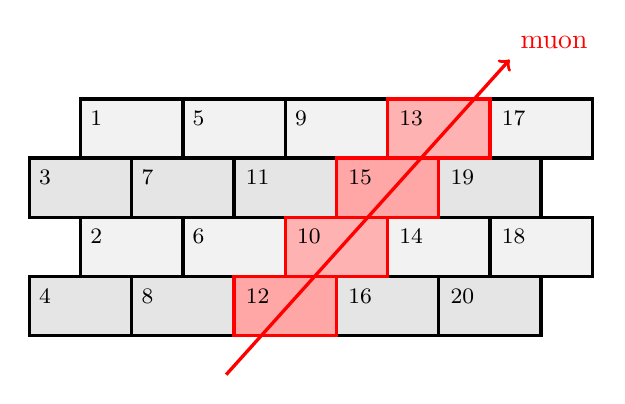
\begin{tikzpicture}

    % lower layer
    \filldraw[color=black, fill=black!10, very thick] (0.0,0.0) rectangle + (1.3,0.75);
    \filldraw[color=black, fill=black!10, very thick] (1.3,0.0) rectangle + (1.3,0.75);
    
    \filldraw[color=black, fill=black!10, very thick] (3.9,0.0) rectangle + (1.3,0.75);
    \filldraw[color=black, fill=black!10, very thick] (5.2,0.0) rectangle + (1.3,0.75);

    \node at (0.2,0.5) {\footnotesize $4$}; 
    \node at (1.5,0.5) {\footnotesize $8$};
    
    \node at (4.2,0.5) {\footnotesize $16$};
    \node at (5.5,0.5) {\footnotesize $20$};
 
    % second layer
    \filldraw[color=black, fill=black!5, very thick] (0.65,0.75) rectangle + (1.3,0.75);
    \filldraw[color=black, fill=black!5, very thick] (1.95,0.75) rectangle + (1.3,0.75);
    \filldraw[color=black, fill=black!5, very thick] (3.25,0.75) rectangle + (1.3,0.75);
    \filldraw[color=black, fill=black!5, very thick] (4.55,0.75) rectangle + (1.3,0.75);
    \filldraw[color=black, fill=black!5, very thick] (5.85,0.75) rectangle + (1.3,0.75);

    \node at (0.2+0.65,0.5+0.75) {\footnotesize $2$}; 
    \node at (1.5+0.65,0.5+0.75) {\footnotesize $6$};
    
    \node at (4.2+0.65,0.5+0.75) {\footnotesize $14$};
    \node at (5.5+0.65,0.5+0.75) {\footnotesize $18$};

    % third layer
    \filldraw[color=black, fill=black!10, very thick] (0.0,1.5) rectangle + (1.3,0.75);
    \filldraw[color=black, fill=black!10, very thick] (1.3,1.5) rectangle + (1.3,0.75);
    \filldraw[color=black, fill=black!10, very thick] (2.6,1.5) rectangle + (1.3,0.75);
    
    \filldraw[color=black, fill=black!10, very thick] (5.2,1.5) rectangle + (1.3,0.75);

    \node at (0.2,2.0) {\footnotesize $3$}; 
    \node at (1.5,2.0) {\footnotesize $7$};
    \node at (2.9,2.0) {\footnotesize $11$};
    
    \node at (5.5,2.0) {\footnotesize $19$};

    % upper layer
    \filldraw[color=black, fill=black!5, very thick] (0.65,2.25) rectangle + (1.3,0.75);
    \filldraw[color=black, fill=black!5, very thick] (1.95,2.25) rectangle + (1.3,0.75);
    \filldraw[color=black, fill=black!5, very thick] (3.25,2.25) rectangle + (1.3,0.75);

    \filldraw[color=black, fill=black!5, very thick] (5.85,2.25) rectangle + (1.3,0.75);

    \node at (0.2+0.65,2.0+0.75) {\footnotesize $1$}; 
    \node at (1.5+0.65,2.0+0.75) {\footnotesize $5$};
    \node at (2.8+0.65,2.0+0.75) {\footnotesize $9$};
    
    \node at (5.5+0.65,2.0+0.75) {\footnotesize $17$};
       
    % muon track
    \filldraw[color=red, fill=red!30, very thick] (4.55,2.25) rectangle + (1.3,0.75);
    \node at (4.2+0.65,2.0+0.75) {\footnotesize $13$};

    \filldraw[color=red, fill=red!35, very thick] (3.9,1.5) rectangle + (1.3,0.75);
    \node at (4.2,2.0) {\footnotesize $15$};

    \filldraw[color=red, fill=red!30, very thick] (3.25,0.75) rectangle + (1.3,0.75);
    \node at (2.9+0.65,0.5+0.75) {\footnotesize $10$};

    \filldraw[color=red, fill=red!35, very thick] (2.6,0.0) rectangle + (1.3,0.75);
    \node at (2.9,0.5) {\footnotesize $12$};

    \draw[color=red, very thick, ->] (2.5,-0.5) -- (6.1,3.5) node[above right] {muon};
     



        
\end{tikzpicture}